\documentclass[supercite]{Experimental_Report}

\title{~~~~~~新生实践课~~~~~~}
\author{王李超}
\school{计算机科学与技术学院}
\classnum{CS启明2401}
\stunum{U202414887}
\instructor{范晔斌} % 李平、孙伟平、范晔斌、陈加忠
\date{2024年12月1日}

\usepackage{algorithm, multirow}
\usepackage{algpseudocode}
\usepackage{amsmath}
\usepackage{amsthm}
\usepackage{framed}
\usepackage{mathtools}
\usepackage{subcaption}
\usepackage{xltxtra} %提供了针对XeTeX的改进并且加入了XeTeX的LOGO, 自动调用xunicode宏包(提供Unicode字符宏)
\usepackage{bm}
\usepackage{tikz}
\usepackage{tikzscale}
\usepackage{pgfplots}
%\usepackage{enumerate}

\pgfplotsset{compat=1.16}

\newcommand{\cfig}[3]{
  \begin{figure}[htb]
    \centering
    \includegraphics[width=#2\textwidth]{images/#1.tikz}
    \caption{#3}
    \label{fig:#1}
  \end{figure}
}

\newcommand{\sfig}[3]{
  \begin{subfigure}[b]{#2\textwidth}
    \includegraphics[width=\textwidth]{images/#1.tikz}
    \caption{#3}
    \label{fig:#1}
  \end{subfigure}
}

\newcommand{\xfig}[3]{
  \begin{figure}[htb]
    \centering
    #3
    \caption{#2}
    \label{fig:#1}
  \end{figure}
}

\newcommand{\rfig}[1]{\autoref{fig:#1}}
\newcommand{\ralg}[1]{\autoref{alg:#1}}
\newcommand{\rthm}[1]{\autoref{thm:#1}}
\newcommand{\rlem}[1]{\autoref{lem:#1}}
\newcommand{\reqn}[1]{\autoref{eqn:#1}}
\newcommand{\rtbl}[1]{\autoref{tbl:#1}}

\algnewcommand\Null{\textsc{null }}
\algnewcommand\algorithmicinput{\textbf{Input:}}
\algnewcommand\Input{\item[\algorithmicinput]}
\algnewcommand\algorithmicoutput{\textbf{Output:}}
\algnewcommand\Output{\item[\algorithmicoutput]}
\algnewcommand\algorithmicbreak{\textbf{break}}
\algnewcommand\Break{\algorithmicbreak}
\algnewcommand\algorithmiccontinue{\textbf{continue}}
\algnewcommand\Continue{\algorithmiccontinue}
\algnewcommand{\LeftCom}[1]{\State $\triangleright$ #1}

\newtheorem{thm}{定理}[section]
\newtheorem{lem}{引理}[section]

\colorlet{shadecolor}{black!15}

\theoremstyle{definition}
\newtheorem{alg}{算法}[section]

\def\thmautorefname~#1\null{定理~#1~\null}
\def\lemautorefname~#1\null{引理~#1~\null}
\def\algautorefname~#1\null{算法~#1~\null}

\begin{document}

\maketitle

\clearpage

\pagenumbering{Roman}

\tableofcontents[level=2]
\clearpage

\pagenumbering{arabic}

\section{网页整体框架}

图\ref{fig1-1}这个网页的整体框架使用HTML与CSS实现,结构清晰简洁,包含头部、主体内容和底部三个主要部分。头部部分通过`<header>`标签呈现,显示网站标题“王李超的个人主页”,背景为黑色半透明,文字居中,视觉效果突出。主体内容区域由一个`<div>`容器构成,采用Flexbox布局,使内容水平居中对齐,容器内放置了五个链接盒子,分别通向“个人经历”“喜欢的音乐”“我的Steam”“Github主页”和“我的资源”页面。每个链接盒子有独特的背景图、文字说明,并添加了悬停时的动画效果,如放大、阴影变化及模糊背景图变清晰,提升交互体验。底部区域由`<footer>`标签定义,显示欢迎语和简单介绍,同样采用黑色半透明背景,使整体风格一致。整个页面的布局通过CSS控制,使网页在不同屏幕设备上自适应,从而提供良好的用户体验,整体风格现代、简洁而不失个性。
% \begin{enumerate}
% \renewcommand{\labelenumi}{\theenumi)}
% 	\item C++
% 	\item Java
% 	\item HTML
% \end{enumerate}

\begin{figure}[htb] % here top bottom
	\begin{center}
		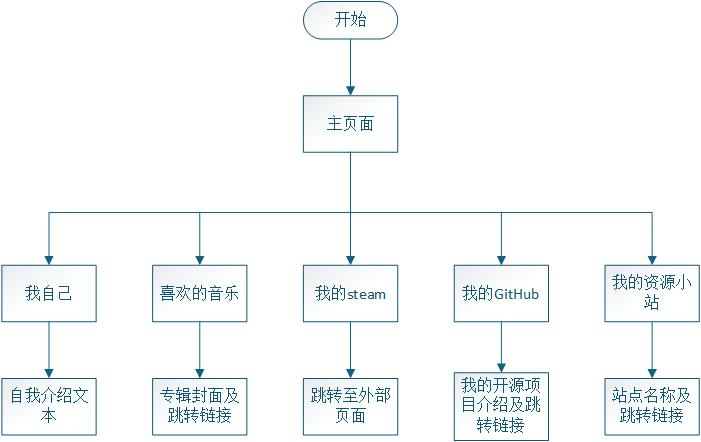
\includegraphics[scale=0.80]{images/1-1.jpg}
		\caption{网页整体框架举例}
		\label{fig1-1}
	\end{center}
\end{figure}

\newpage

\section{主页设计}

1. 头部结构:头部区域使用`<header>`标签,显示网页标题“王李超的个人主页”,文字居中,采用白色字体和黑色透明背景。此设计增加了标题的视觉层次感,同时保持整体简洁大方。

2. 主体内容布局:主体区域通过一个`<div class="content">`容器承载,主要功能是展示五个链接盒子。每个盒子分别对应“个人经历”“喜欢的音乐”“我的Steam”“Github主页”和“我的资源”五个子页面,链接直观明了,方便导航。

3. 盒子设计:每个链接盒子都采用白色半透明背景,带有圆角和阴影效果。盒子内文字居中显示,使用粗体设计,整体呈现干净、现代的风格。盒子宽高比为黄金比例,使视觉效果更加和谐。

4. 动态交互效果:盒子设计中加入悬停时的动画效果,通过CSS实现。当鼠标悬停时,盒子会放大并增强阴影效果,同时背景图片从模糊变为清晰,使用户体验更加生动且有趣。

5. 布局实现:整个页面使用Flexbox布局,确保内容在不同设备和屏幕尺寸下都能保持良好的自适应效果。盒子排列居中,水平间距均匀,增强页面的对称性和美观度。

6. 底部结构:底部区域使用`<footer>`标签,展示欢迎信息和个人简介。采用黑色透明背景,与头部设计保持一致,文字居中排布,简洁而不失信息量。

7. 色彩与背景:页面整体以深色为主,通过透明背景与半透明盒子形成视觉对比。同时,页面背景为全屏图像,增加页面的层次感和视觉吸引力,使整体风格更具现代感。

8. 响应式设计:通过`<meta>`标签设置视口,使页面能自动适应各种设备屏幕尺寸,优化了移动设备的浏览体验,从而增强了网站的兼容性与实用性。

9. 设计思路总结:整个页面设计追求简洁、现代和互动性,突出用户体验。通过色彩、动画效果及布局优化,使用户在视觉和交互上都能感受到良好的体验。请见图\ref{fig2-1}。


\begin{figure}[htb]
	\begin{center}
		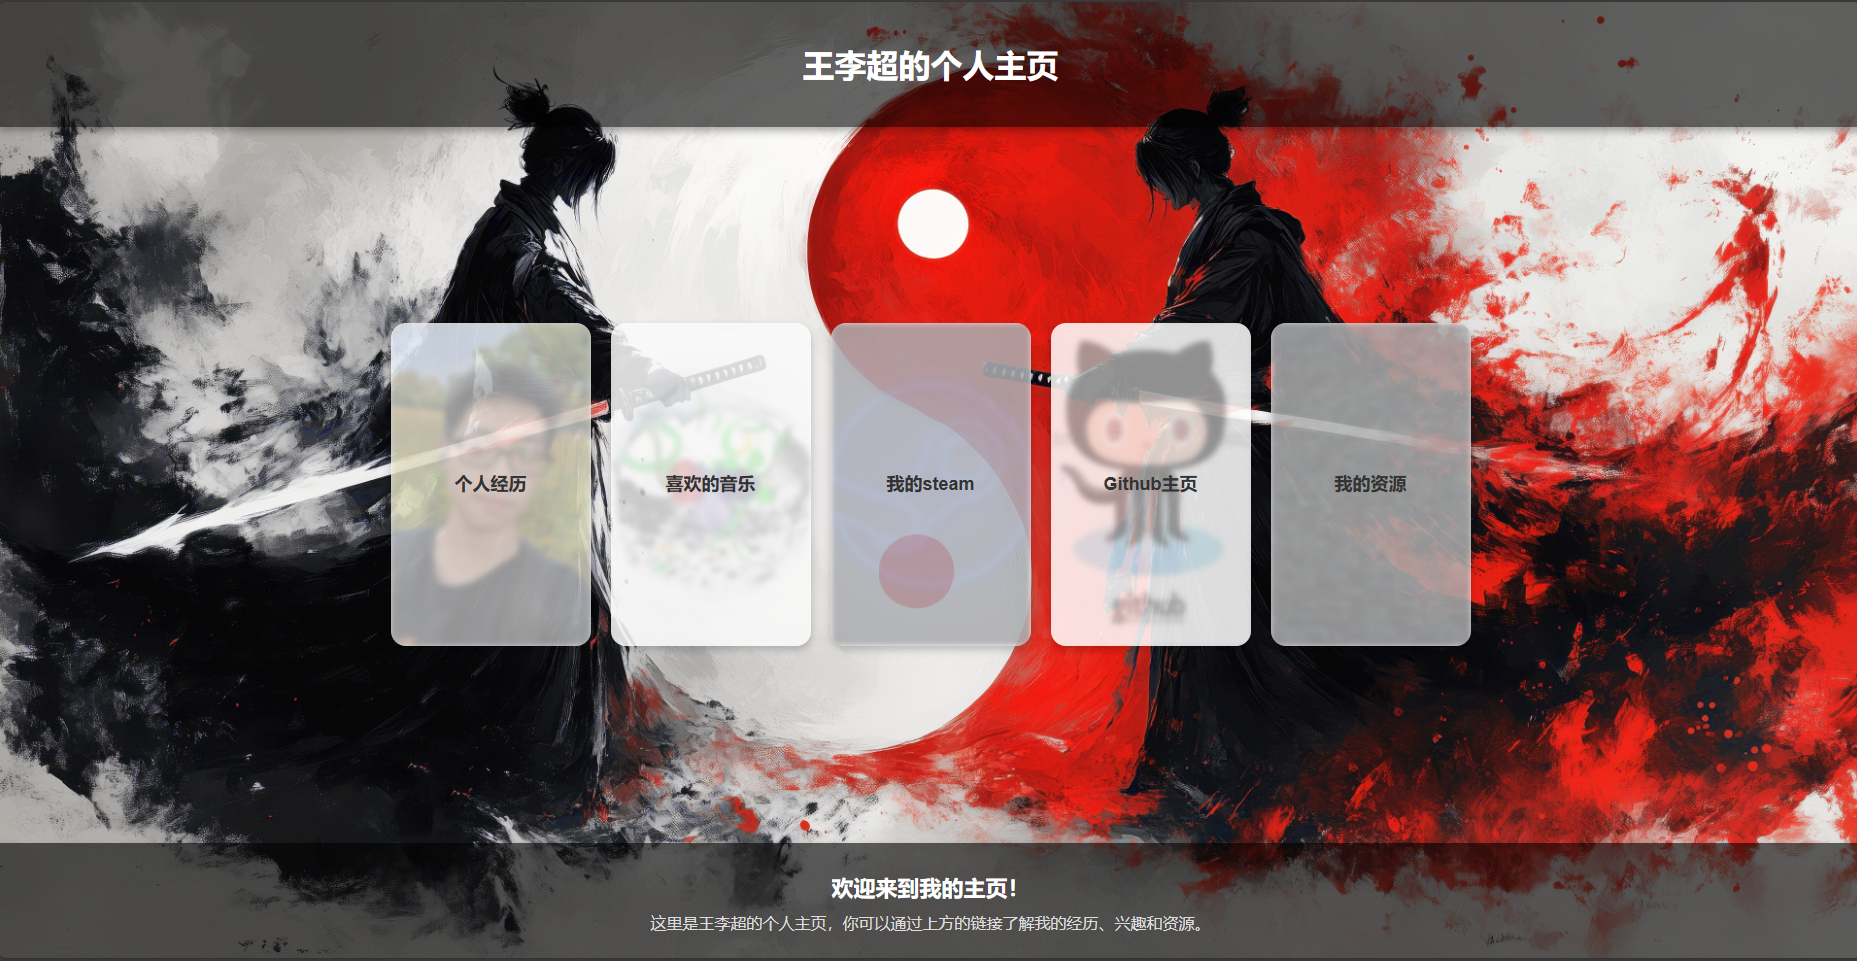
\includegraphics[scale=0.30]{images/2-1.png}
		\caption{主页举例}
		\label{fig2-1}
	\end{center}
\end{figure}

\newpage

\section{分页面设计}

给出分页面截图,描述主要设计思路等。给出分页面截图,描述主要设计思路等。给出分页面截图,描述主要设计思路等。给出分页面截图,描述主要设计思路等。

\subsection{页面1 (个人信息页面设计)}

该页面以展示“王李超的个人主页 - 个人资料”为主题,设计中遵循简洁、直观的原则,整体风格统一,易于用户浏览。页面头部使用\texttt{<header>}标签定义,标题“王李超的个人主页 - 个人资料”居中显示,采用黑色半透明背景与白色文字,形成简洁大方的视觉效果。通过适当的\texttt{padding},提升标题的可读性和整体页面的舒适感。主体部分通过\texttt{<div class="content">}容器包裹,采用Flexbox布局,使内容在垂直与水平方向居中对齐,确保在不同屏幕尺寸下依然保持居中状态。个人信息部分通过\texttt{<div class="project-details">}展示,每条信息单独使用\texttt{<div class="line">}包裹,增加白色字体与半透明背景,增强可读性和视觉层次感。每条信息块添加圆角、内边距及阴影效果,使用\texttt{box-shadow}提升立体感。此外,通过\texttt{white-space: nowrap}保证每段信息一行显示,使排版整洁。页面底部提供了跳转至Github的链接,用户点击即可访问相关资源。底部使用\texttt{<footer>}标签定义,背景风格与头部保持一致,采用黑色透明背景、白色文字,整体视觉风格和谐统一。通过\texttt{text-align: center}使欢迎信息与简要说明居中排列,进一步增强整体视觉的均衡感。为确保页面在各类设备上的适应性,通过\texttt{<meta>}视口设置,实现内容自适应布局。同时,Flexbox布局使各元素在不同屏幕尺寸下均保持居中,提高用户体验。文字内容设置最大宽度为视口宽度的100\%,防止内容溢出,提升排版稳定性。整体设计考虑了美观与实用性,确保在信息传递的同时,保持页面的简洁与高效。


\begin{shaded*}
	\begin{alg}{网页源代码}
		\label{alg:1}
		\begin{algorithmic}
			\State \textbf{<!DOCTYPE html>}
			\State \textbf{<html lang="zh-CN">}
			\State \ \ \ \ \textbf{<head>}
			\State \ \ \ \ \ \ \ \ \ \textbf{<meta charset="UTF-8">}
			\State \ \ \ \ \ \ \ \ \ \textbf{<meta name="viewport" content="width=device-width, initial-scale=1.0">}
			\State \ \ \ \ \ \ \ \ \ \textbf{<title>王李超的个人主页 - 个人资料</title>}
			\State \ \ \ \ \ \ \ \ \ \textbf{<link rel="icon" href="../images/favicon.ico" type="image/x-icon">}
			\State \ \ \ \ \ \ \ \ \ \textbf{<style>}
			\State \ \ \ \ \ \ \ \ \ \ \ \textbf{body \{} \texttt{font-family: Arial, sans-serif;}
			\State \ \ \ \ \ \ \ \ \ \ \ \ \textbf{background-image: url('experience\_background.png');}
			\State \ \ \ \ \ \ \ \ \ \ \ \ \textbf{background-size: cover;}
			\State \ \ \ \ \ \ \ \ \ \ \ \ \textbf{background-position: center;}
			\State \ \ \ \ \ \ \ \ \ \ \ \ \textbf{background-attachment: fixed;}
			\State \ \ \ \ \ \ \ \ \ \ \ \ \textbf{color: hsl(0, 0\%, 0\%); }
			\State \ \ \ \ \ \ \ \ \ \ \ \ \textbf{display: flex;}
			\State \ \ \ \ \ \ \ \ \ \ \ \ \textbf{flex-direction: column;}
			\State \ \ \ \ \ \ \ \ \ \ \ \ \textbf{min-height: 100vh;}
			\State \ \ \ \ \ \ \ \ \ \ \ \textbf{<style>}
			\State \ \ \ \ \textbf{<body>}
			\State \ \ \ \ \ \ \ \ \textbf{<header>}
			\State \ \ \ \ \ \ \ \ \ \ \ \textbf{<h1>王李超的个人主页 - 个人资料</h1>}
			\State \ \ \ \ \ \ \ \ \textbf{</header>}
			\State \ \ \ \ \ \ \ \ \textbf{<div class="content">}
			\State \ \ \ \ \ \ \ \ \ \ \ \textbf{<div class="project-details">}
			\State \ \ \ \ \ \ \ \ \ \ \ \ \textbf{<div class="line">姓名:王李超</div>}
			\State \ \ \ \ \ \ \ \ \ \ \ \ \textbf{<div class="line">一看就是男的</div>}
			\State \ \ \ \ \ \ \ \ \ \ \ \ \textbf{<div class="line">广涉猎而不精</div>}
			\State \ \ \ \ \ \ \ \ \ \ \ \ \textbf{<div class="line">现在正在被学习折磨</div>}
			\State \ \ \ \ \ \ \ \ \ \ \ \ \textbf{<div class="line">暂时还没有项目在做</div>}
			\State \ \ \ \ \ \ \ \ \ \ \ \ \textbf{<div class="line">若想看我写的代码请移步<a href="web/github.html">Github</a></div>}
			\State \ \ \ \ \ \ \ \ \ \ \ \textbf{</div>}
			\State \ \ \ \ \ \ \ \ \textbf{</div>}
			\State \ \ \ \ \ \ \ \ \textbf{<footer>}
			\State \ \ \ \ \ \ \ \ \ \ \ \textbf{<h2>欢迎来到我的主页!</h2>}
			\State \ \ \ \ \ \ \ \ \ \ \ \textbf{<p>这里是王李超的个人主页,你可以通过上方的链接了解我的经历。</p>}
			\State \ \ \ \ \ \ \ \ \textbf{</footer>}
			\State \textbf{</body>}
			\State \textbf{</html>}
		\end{algorithmic}
	\end{alg}
	\end{shaded*}
	

\subsection{页面2 (每个页面以主要内容起标题名称即可)}

给出分页面截图,描述主要设计思路等。给出分页面截图,描述主要设计思路等。给出分页面截图,描述主要设计思路等。给出分页面截图,描述主要设计思路等。给出分页面截图,描述主要设计思路等。给出分页面截图,描述主要设计思路等。给出分页面截图,描述主要设计思路等。给出分页面截图,描述主要设计思路等。给出分页面截图,描述主要设计思路等。给出分页面截图,描述主要设计思路等。给出分页面截图,描述主要设计思路等。


如果实验报告中要用到算法伪代码,请参考算法\ref{alg:1},也可以参考算法\ref{alg:2}。如果实验报告中要用到算法伪代码,请参考算法\ref{alg:1},也可以参考算法\ref{alg:2}。如果实验报告中要用到算法伪代码,请参考算法\ref{alg:1},也可以参考算法\ref{alg:2}。如果实验报告中要用到算法伪代码,请参考算法\ref{alg:1},也可以参考算法\ref{alg:2}。

\begin{algorithm}[h] 
	\caption{一个更复杂算法}
	\begin{algorithmic}[1]
		\State Initialization: $I_{xy}$, $z_{f}=Zeros(128, 128)$; 
		\For{$0\leq n \textless N$}
		\State $i=\lfloor x_n \rfloor+64$, $j=\lfloor y_n \rfloor + 64$
		\If{$z_n<0$ and $|z_n|>|z_{f}(i,j)|$};
		\State $z_{f}(i,j)=z_n$;
		\EndIf
		\State $I_{xy}(i,j)=z_{f}(i,j)$;
		\EndFor 
	\end{algorithmic}\label{alg:2}
\end{algorithm}

\subsection{页面3 (每个页面以主要内容起标题名称即可)}

给出分页面截图,描述主要设计思路等。给出分页面截图,描述主要设计思路等。给出分页面截图,描述主要设计思路等。给出分页面截图,描述主要设计思路等。给出分页面截图,描述主要设计思路等。给出分页面截图,描述主要设计思路等。给出分页面截图,描述主要设计思路等。给出分页面截图,描述主要设计思路等。给出分页面截图,描述主要设计思路等。给出分页面截图,描述主要设计思路等。给出分页面截图,描述主要设计思路等。

\subsection{页面4 (每个页面以主要内容起标题名称即可)}

给出分页面截图,描述主要设计思路等。给出分页面截图,描述主要设计思路等。给出分页面截图,描述主要设计思路等。给出分页面截图,描述主要设计思路等。给出分页面截图,描述主要设计思路等。给出分页面截图,描述主要设计思路等。给出分页面截图,描述主要设计思路等。给出分页面截图,描述主要设计思路等。给出分页面截图,描述主要设计思路等。给出分页面截图,描述主要设计思路等。给出分页面截图,描述主要设计思路等。

\newpage

\section{网页设计小结}

描述网页的设计和实现过程中遇到的问题及如何解决。描述网页的设计和实现过程中遇到的问题及如何解决。描述网页的设计和实现过程中遇到的问题及如何解决。描述网页的设计和实现过程中遇到的问题及如何解决。描述网页的设计和实现过程中遇到的问题及如何解决。描述网页的设计和实现过程中遇到的问题及如何解决。描述网页的设计和实现过程中遇到的问题及如何解决。描述网页的设计和实现过程中遇到的问题及如何解决。描述网页的设计和实现过程中遇到的问题及如何解决。

描述网页的设计和实现过程中遇到的问题及如何解决。描述网页的设计和实现过程中遇到的问题及如何解决。描述网页的设计和实现过程中遇到的问题及如何解决。描述网页的设计和实现过程中遇到的问题及如何解决。描述网页的设计和实现过程中遇到的问题及如何解决。描述网页的设计和实现过程中遇到的问题及如何解决。描述网页的设计和实现过程中遇到的问题及如何解决。描述网页的设计和实现过程中遇到的问题及如何解决。描述网页的设计和实现过程中遇到的问题及如何解决。

描述网页的设计和实现过程中遇到的问题及如何解决。描述网页的设计和实现过程中遇到的问题及如何解决。描述网页的设计和实现过程中遇到的问题及如何解决。描述网页的设计和实现过程中遇到的问题及如何解决。描述网页的设计和实现过程中遇到的问题及如何解决。描述网页的设计和实现过程中遇到的问题及如何解决。描述网页的设计和实现过程中遇到的问题及如何解决。描述网页的设计和实现过程中遇到的问题及如何解决。描述网页的设计和实现过程中遇到的问题及如何解决。

描述网页的设计和实现过程中遇到的问题及如何解决。描述网页的设计和实现过程中遇到的问题及如何解决。描述网页的设计和实现过程中遇到的问题及如何解决。描述网页的设计和实现过程中遇到的问题及如何解决。描述网页的设计和实现过程中遇到的问题及如何解决。描述网页的设计和实现过程中遇到的问题及如何解决。描述网页的设计和实现过程中遇到的问题及如何解决。描述网页的设计和实现过程中遇到的问题及如何解决。描述网页的设计和实现过程中遇到的问题及如何解决。

\newpage

\section{课程的收获和建议}

描述通过学习该专题,有何收获,有何建议,如某专题可适当减少讲授时间、某专题可适当增加讲授内容和时间等。描述通过学习该专题,有何收获,有何建议,如某专题可适当减少讲授时间、某专题可适当增加讲授内容和时间等。描述通过学习该专题,有何收获,有何建议,如某专题可适当减少讲授时间、某专题可适当增加讲授内容和时间等。描述通过学习该专题,有何收获,有何建议,如某专题可适当减少讲授时间、某专题可适当增加讲授内容和时间等。

\subsection{计算机基础知识}

描述通过学习计算机基础知识专题,有何收获,有何建议,如某专题可适当减少讲授时间、某专题可适当增加讲授内容和时间等。描述网页的设计和实现过程中遇到的问题及如何解决。描述网页的设计和实现过程中遇到的问题及如何解决。描述网页的设计和实现过程中遇到的问题及如何解决。描述网页的设计和实现过程中遇到的问题及如何解决。描述网页的设计和实现过程中遇到的问题及如何解决。描述网页的设计和实现过程中遇到的问题及如何解决。描述网页的设计和实现过程中遇到的问题及如何解决。描述网页的设计和实现过程中遇到的问题及如何解决。

\subsection{文档撰写工具LaTeX}

描述通过学习文档撰写工具LaTeX专题,有何收获,有何建议,如某专题可适当减少讲授时间、某专题可适当增加讲授内容和时间等。描述通过学习文档撰写工具LaTeX专题,有何收获,有何建议,如某专题可适当减少讲授时间、某专题可适当增加讲授内容和时间等。

\subsection{编程工具Python}

描述通过学习编程工具Python专题,有何收获,有何建议,如某专题可适当减少讲授时间、某专题可适当增加讲授内容和时间等。描述通过学习编程工具Python专题,有何收获,有何建议,如某专题可适当减少讲授时间、某专题可适当增加讲授内容和时间等。

\subsection{图像设计软件Photoshop}

描述通过学习计算机基础知识专题,有何收获,有何建议,如某专题可适当减少讲授时间、某专题可适当增加讲授内容和时间等。描述通过学习计算机基础知识专题,有何收获,有何建议,如某专题可适当减少讲授时间、某专题可适当增加讲授内容和时间等。

\subsection{版本管理软件Git}

描述通过学习图像设计软件Photoshop专题,有何收获,有何建议,如某专题可适当减少讲授时间、某专题可适当增加讲授内容和时间等。描述通过学习图像设计软件Photoshop专题,有何收获,有何建议,如某专题可适当减少讲授时间、某专题可适当增加讲授内容和时间等。

\subsection{网页制作Dreamweaver}

描述通过学习网页制作Dreamweaver专题,有何收获,有何建议,如某专题可适当减少讲授时间、某专题可适当增加讲授内容和时间等。描述通过学习网页制作Dreamweaver专题,有何收获,有何建议,如某专题可适当减少讲授时间、某专题可适当增加讲授内容和时间等。


\nocite{*} %% 作用是不对文献进行引用,但可以生成文献列表

%\bibliographystyle{HustGraduPaper}
%\bibliography{HustGraduPaper}

\end{document}
